% Created by tikzDevice version 0.12.6 on 2024-03-15 15:16:39
% !TEX encoding = UTF-8 Unicode
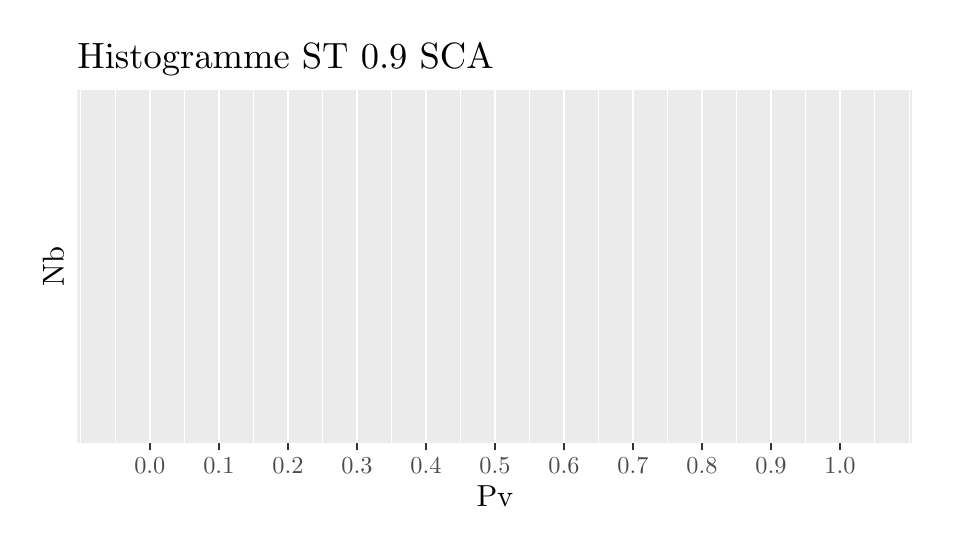
\begin{tikzpicture}[x=1pt,y=1pt]
\definecolor{fillColor}{RGB}{255,255,255}
\path[use as bounding box,fill=fillColor,fill opacity=0.00] (0,0) rectangle (325.21,180.67);
\begin{scope}
\path[clip] (  0.00,  0.00) rectangle (325.21,180.67);
\definecolor{drawColor}{RGB}{255,255,255}
\definecolor{fillColor}{RGB}{255,255,255}

\path[draw=drawColor,line width= 0.6pt,line join=round,line cap=round,fill=fillColor] (  0.00,  0.00) rectangle (325.21,180.68);
\end{scope}
\begin{scope}
\path[clip] ( 17.96, 30.69) rectangle (319.71,158.02);
\definecolor{fillColor}{gray}{0.92}

\path[fill=fillColor] ( 17.96, 30.69) rectangle (319.71,158.02);
\definecolor{drawColor}{RGB}{255,255,255}

\path[draw=drawColor,line width= 0.3pt,line join=round] ( 19.21, 30.69) --
	( 19.21,158.02);

\path[draw=drawColor,line width= 0.3pt,line join=round] ( 31.68, 30.69) --
	( 31.68,158.02);

\path[draw=drawColor,line width= 0.3pt,line join=round] ( 56.62, 30.69) --
	( 56.62,158.02);

\path[draw=drawColor,line width= 0.3pt,line join=round] ( 81.56, 30.69) --
	( 81.56,158.02);

\path[draw=drawColor,line width= 0.3pt,line join=round] (106.49, 30.69) --
	(106.49,158.02);

\path[draw=drawColor,line width= 0.3pt,line join=round] (131.43, 30.69) --
	(131.43,158.02);

\path[draw=drawColor,line width= 0.3pt,line join=round] (156.37, 30.69) --
	(156.37,158.02);

\path[draw=drawColor,line width= 0.3pt,line join=round] (181.31, 30.69) --
	(181.31,158.02);

\path[draw=drawColor,line width= 0.3pt,line join=round] (206.25, 30.69) --
	(206.25,158.02);

\path[draw=drawColor,line width= 0.3pt,line join=round] (231.18, 30.69) --
	(231.18,158.02);

\path[draw=drawColor,line width= 0.3pt,line join=round] (256.12, 30.69) --
	(256.12,158.02);

\path[draw=drawColor,line width= 0.3pt,line join=round] (281.06, 30.69) --
	(281.06,158.02);

\path[draw=drawColor,line width= 0.3pt,line join=round] (306.00, 30.69) --
	(306.00,158.02);

\path[draw=drawColor,line width= 0.3pt,line join=round] (318.47, 30.69) --
	(318.47,158.02);

\path[draw=drawColor,line width= 0.6pt,line join=round] ( 44.15, 30.69) --
	( 44.15,158.02);

\path[draw=drawColor,line width= 0.6pt,line join=round] ( 69.09, 30.69) --
	( 69.09,158.02);

\path[draw=drawColor,line width= 0.6pt,line join=round] ( 94.03, 30.69) --
	( 94.03,158.02);

\path[draw=drawColor,line width= 0.6pt,line join=round] (118.96, 30.69) --
	(118.96,158.02);

\path[draw=drawColor,line width= 0.6pt,line join=round] (143.90, 30.69) --
	(143.90,158.02);

\path[draw=drawColor,line width= 0.6pt,line join=round] (168.84, 30.69) --
	(168.84,158.02);

\path[draw=drawColor,line width= 0.6pt,line join=round] (193.78, 30.69) --
	(193.78,158.02);

\path[draw=drawColor,line width= 0.6pt,line join=round] (218.72, 30.69) --
	(218.72,158.02);

\path[draw=drawColor,line width= 0.6pt,line join=round] (243.65, 30.69) --
	(243.65,158.02);

\path[draw=drawColor,line width= 0.6pt,line join=round] (268.59, 30.69) --
	(268.59,158.02);

\path[draw=drawColor,line width= 0.6pt,line join=round] (293.53, 30.69) --
	(293.53,158.02);
\end{scope}
\begin{scope}
\path[clip] (  0.00,  0.00) rectangle (325.21,180.67);
\definecolor{drawColor}{gray}{0.20}

\path[draw=drawColor,line width= 0.6pt,line join=round] ( 44.15, 27.94) --
	( 44.15, 30.69);

\path[draw=drawColor,line width= 0.6pt,line join=round] ( 69.09, 27.94) --
	( 69.09, 30.69);

\path[draw=drawColor,line width= 0.6pt,line join=round] ( 94.03, 27.94) --
	( 94.03, 30.69);

\path[draw=drawColor,line width= 0.6pt,line join=round] (118.96, 27.94) --
	(118.96, 30.69);

\path[draw=drawColor,line width= 0.6pt,line join=round] (143.90, 27.94) --
	(143.90, 30.69);

\path[draw=drawColor,line width= 0.6pt,line join=round] (168.84, 27.94) --
	(168.84, 30.69);

\path[draw=drawColor,line width= 0.6pt,line join=round] (193.78, 27.94) --
	(193.78, 30.69);

\path[draw=drawColor,line width= 0.6pt,line join=round] (218.72, 27.94) --
	(218.72, 30.69);

\path[draw=drawColor,line width= 0.6pt,line join=round] (243.65, 27.94) --
	(243.65, 30.69);

\path[draw=drawColor,line width= 0.6pt,line join=round] (268.59, 27.94) --
	(268.59, 30.69);

\path[draw=drawColor,line width= 0.6pt,line join=round] (293.53, 27.94) --
	(293.53, 30.69);
\end{scope}
\begin{scope}
\path[clip] (  0.00,  0.00) rectangle (325.21,180.67);
\definecolor{drawColor}{gray}{0.30}

\node[text=drawColor,anchor=base,inner sep=0pt, outer sep=0pt, scale=  0.88] at ( 44.15, 19.68) {0.0};

\node[text=drawColor,anchor=base,inner sep=0pt, outer sep=0pt, scale=  0.88] at ( 69.09, 19.68) {0.1};

\node[text=drawColor,anchor=base,inner sep=0pt, outer sep=0pt, scale=  0.88] at ( 94.03, 19.68) {0.2};

\node[text=drawColor,anchor=base,inner sep=0pt, outer sep=0pt, scale=  0.88] at (118.96, 19.68) {0.3};

\node[text=drawColor,anchor=base,inner sep=0pt, outer sep=0pt, scale=  0.88] at (143.90, 19.68) {0.4};

\node[text=drawColor,anchor=base,inner sep=0pt, outer sep=0pt, scale=  0.88] at (168.84, 19.68) {0.5};

\node[text=drawColor,anchor=base,inner sep=0pt, outer sep=0pt, scale=  0.88] at (193.78, 19.68) {0.6};

\node[text=drawColor,anchor=base,inner sep=0pt, outer sep=0pt, scale=  0.88] at (218.72, 19.68) {0.7};

\node[text=drawColor,anchor=base,inner sep=0pt, outer sep=0pt, scale=  0.88] at (243.65, 19.68) {0.8};

\node[text=drawColor,anchor=base,inner sep=0pt, outer sep=0pt, scale=  0.88] at (268.59, 19.68) {0.9};

\node[text=drawColor,anchor=base,inner sep=0pt, outer sep=0pt, scale=  0.88] at (293.53, 19.68) {1.0};
\end{scope}
\begin{scope}
\path[clip] (  0.00,  0.00) rectangle (325.21,180.67);
\definecolor{drawColor}{RGB}{0,0,0}

\node[text=drawColor,anchor=base,inner sep=0pt, outer sep=0pt, scale=  1.10] at (168.84,  7.64) {Pv};
\end{scope}
\begin{scope}
\path[clip] (  0.00,  0.00) rectangle (325.21,180.67);
\definecolor{drawColor}{RGB}{0,0,0}

\node[text=drawColor,rotate= 90.00,anchor=base,inner sep=0pt, outer sep=0pt, scale=  1.10] at ( 13.08, 94.35) {Nb};
\end{scope}
\begin{scope}
\path[clip] (  0.00,  0.00) rectangle (325.21,180.67);
\definecolor{drawColor}{RGB}{0,0,0}

\node[text=drawColor,anchor=base west,inner sep=0pt, outer sep=0pt, scale=  1.32] at ( 17.96,166.08) {Histogramme ST 0.9 SCA};
\end{scope}
\end{tikzpicture}
